\documentclass[10pt,a4paper]{article}
\usepackage[paper=a4paper,left=30mm,right=30mm,top=30mm,bottom=30mm]{geometry} 
\usepackage[english, ngerman]{babel}
\usepackage[utf8]{inputenc}
\usepackage[colorlinks=false]{hyperref}
\usepackage{tabularx}
\usepackage{listings}
\usepackage{graphicx}
\usepackage{float}
\usepackage{fancyhdr}
\usepackage{color}

\definecolor{javared}{rgb}{0.6,0,0} % for strings
\definecolor{javagreen}{rgb}{0.25,0.5,0.35} % comments
\definecolor{javapurple}{rgb}{0.5,0,0.35} % keywords
\definecolor{javadocblue}{rgb}{0.25,0.35,0.75} % javadoc
 
\lstset{
language=Java,
basicstyle=\ttfamily,
keywordstyle=\color{javapurple}\bfseries,
stringstyle=\color{javared},
commentstyle=\color{javagreen},
morecomment=[s][\color{javadocblue}]{/**}{*/},
numbers=left,
numberstyle=\tiny\color{black},
stepnumber=1,
numbersep=10pt,
tabsize=4,
showspaces=false,
showstringspaces=false}

\pagestyle{fancy}

\renewcommand{\headrulewidth}{0pt}
\lhead{}%{\includegraphics[width=80mm]{../logo.png}}
\chead{}
\rhead{}
\lfoot{Gruppe White}
\cfoot{}
\rfoot{\thepage}

\renewcommand{\arraystretch}{1.3}

\begin{document}
\section*{State pattern (Zustandsmuster)}
%
\subsection*{Hintergrund}
%
Das Zustands-Entwurfsmuster ist eine Methode zur Modellierung von zustandsabhängigen Verhalten eines Objekts, resp. es soll sein äusseres Verhalten zur Laufzeit aufgrund seines Zustands ändern. Das Verhalten eines Objekts ändert sich entsprechenden seines internen Zustand. Für alle möglichen Zustände wird eine definierte Schnittstelle bereitgestellt. Die Schnittstelle wird für jeden einzelnen Zustand durch eine separate Klasse implementiert.
%
\begin{figure}[H]
  \begin{center}
    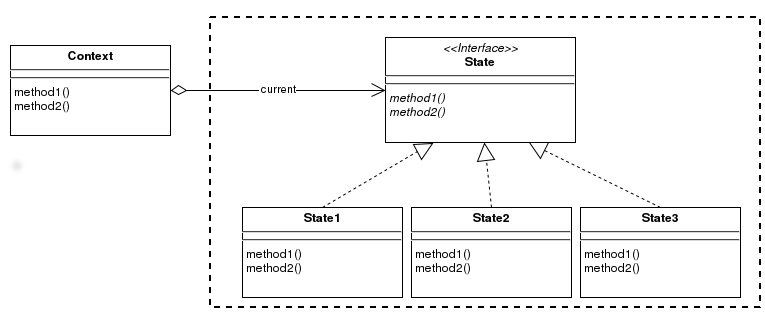
\includegraphics[width=0.95\textwidth]{state-pattern01.png}
    \caption{State pattern}
    \label{fig:state-pattern}
  \end{center}
\end{figure}
%
\subsection*{Vor- und Nachteile}
%
Weitere Zustände und Verhalten können einfach hinzugefügt werden. Die Weiterverwendung der Zustände und bessere Wartbarkeit sind ebenfalls Vorteile. Unleserlichkeit und Unübersichtlichkeit wird entgegen gewirkt, da umfangreiche if-then-else- und switch-Konstrukte vermieden werden.\\ \\
Ein Nachteil ist, das bei einfachen Zustand ein erhöhter Implementierungsaufwand besteht, denn alle Aktionen und Zustände müssen definiert werden. Dies führt zu einer erhöhten Klassenanzahl, da die Schnittstelle komplett implementiert werden muss.
%
\subsection*{Mögliche Implementation}
%
Für eine Türe zeigt nachfolgende Inplementation eine Anwendung des Zustandsmuster. Die Türe hat die folgenden Zustände und Aktionen:
%
\begin{itemize}
  \item offen $\rightarrow$ schliessen
  \item geschlossen $\rightarrow$  abschliessen
  \item verschlossen $\rightarrow$ öffnen
\end{itemize}
%
\begin{figure}[H]
  \begin{center}
    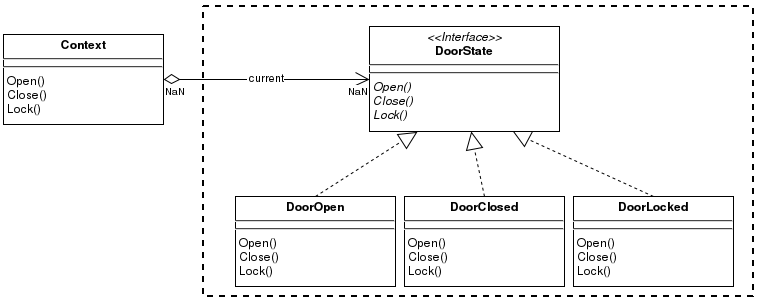
\includegraphics[width=0.95\textwidth]{state-pattern02.png}
    \caption{State pattern}
    \label{fig:door-state}
  \end{center}
\end{figure}
%
Das Interface listet die möglichen Aktionen gemäss der obrigen Aufzählung auf.
%
\begin{lstlisting}[caption={Interface}]
// State of the door
public interface DoorState {
	public String close();
	public String lock();
	public String open();
}
\end{lstlisting}
%
Analog Abbildung \ref{fig:door-state} gibt es drei Zustände und darausfolgende Aktionen.
%
\begin{lstlisting}[caption={Zustand: Türe geöffnet}]
//Concrete State: DoorOpen
public class DoorOpen implements DoorState {
	public String close() {
		return "Can close the door.";
	}

	@Override
	public String lock() {
		return "Can not lock the door.";
	}

	@Override
	public String open() {
		return "Door is already open.";
	}
}
\end{lstlisting}
%
\begin{lstlisting}[caption={Zustand: Türe geschlossen}]
//Concrete State: DoorClosed
public class DoorClosed implements DoorState {
	@Override
	public String lock() {
		return "Lock the door.";
	}

	@Override
	public String close() {
		return "Door is already closed.";
	}

	@Override
	public String open() {
		return "Open the door.";
	}
}
\end{lstlisting}
%
\begin{lstlisting}[caption={Zustand: Türe verschlossen}]
//Concrete State: DoorLocked
public class DoorLocked implements DoorState {
	@Override
	public String open() {
		return "Can open the door. ";
	}

	@Override
	public String close() {
		return "Door is closed.";
	}

	@Override
	public String lock() {
		return "Door is alreay locked.";
	}
}
\end{lstlisting}
%
Die Kontext-Klasse hat eine Verbindung zum Interface.
%
\begin{lstlisting}[caption={Context}]
// Context
public class Door implements DoorState {
	DoorState doorState;

	public Door(DoorState doorState) {
		this.doorState = doorState;
	}

	public void setDoorState(DoorState doorState) {
		this.doorState = doorState;
	}
	
	@Override
	public String close() {
		return doorState.close();
	}

	@Override
	public String lock() {
		return doorState.lock();
	}

	@Override
	public String open() {
		return doorState.open();
	}
}
\end{lstlisting}
%
Die State-Klasse demonstriert die Verwendung.
%
\begin{lstlisting}[caption={State-Klasse}]
public class State {
	public static void main(String[] args) {
		Door door = new Door(new DoorOpen());
		System.out.println("Door is open:");
		System.out.println("- " + door.open());
		System.out.println("- " + door.close());
		System.out.println("- " + door.lock());
		
		door.setDoorState(new DoorClosed());
		System.out.println("Door is closed:");
		System.out.println("- " + door.open());
		System.out.println("- " + door.close());
		System.out.println("- " + door.lock());

		door.setDoorState(new DoorLocked());
		System.out.println("Door is locked:");
		System.out.println("- " + door.open());
		System.out.println("- " + door.close());
		System.out.println("- " + door.lock());
	}
}
\end{lstlisting}
%
Jenach Zustand wird eine andere Aktion ausgeführt. Die Ausgabe zeigt dies.
%
\begin{lstlisting}[caption={Output}]
Door is open:
- Door is already open.
- Can close the door.
- Can not lock the door.
Door is closed:
- Open the door.
- Door is already closed.
- Lock the door.
Door is locked:
- Can open the door. 
- Door is closed.
- Door is alreay locked.
\end{lstlisting}
%
\subsection*{Unsere Implementation}
%

%
\end{document}
